%	PACKAGES AND OTHER DOCUMENT CONFIGURATIONS
%----------------------------------------------------------------------------------------

\documentclass[12pt]{article}
\usepackage{amssymb}
\usepackage[ampersand]{easylist}
\usepackage[danish]{babel}
\usepackage{mathtools}
\usepackage[euler]{textgreek}
\usepackage[numbered,final]{mcode}
\usepackage[utf8x]{inputenc}
\usepackage{amsmath}
\usepackage{graphicx}
\usepackage[colorinlistoftodos]{todonotes}
\usepackage[toc,page]{appendix}
%\usepackage{float}
\usepackage{floatrow} % used for adding "Source" to pictures
\usepackage{hyperref} % used for hyperlinks
\usepackage[all]{hypcap}
\usepackage{bm} % used for bold inline matj
\usepackage{lipsum} % used for lorem lipsum
\usepackage[final]{pdfpages} % used for including PDF's
\usepackage{geometry}
\usepackage{listingsutf8}
\usepackage{listings}
\usepackage{color} %red, green, blue, yellow, cyan, magenta, black, white
\definecolor{mygreen}{RGB}{28,172,0} % color values Red, Green, Blue
\definecolor{mylilas}{RGB}{170,55,241}

\hypersetup{colorlinks=true, linkcolor=black}

\ListProperties(Hide=100, Hang=true, Progressive=3ex, Style*=-- ,
Style2*=$\bullet$ ,Style3*=$\circ$ ,Style4*=\tiny$\blacksquare$ )

% Page margins
\geometry{verbose,tmargin=1in,bmargin=1in,lmargin=1in,rmargin=1in,headsep=0.35in}

\begin{document}
	
	\begin{titlepage}
		
		
		
		\newcommand{\HRule}{\rule{\linewidth}{0.5mm}} % Defines a new command for the horizontal lines, change thickness here
		\setlength{\topmargin}{0in}
		\centering % Center everything on the page
		
		%----------------------------------------------------------------------------------------
		%	HEADING SECTIONS
		%----------------------------------------------------------------------------------------
		\textsc{\LARGE Aarhus universitet}\\[1.5cm] % Name of your university/college
		\textsc{\Large Smartphone Applikationer}\\[0.5cm] % Major heading such as course name
		\textsc{\large 6. Semester}\\[0.5cm] % Minor heading such as course title
		
		%----------------------------------------------------------------------------------------
		%	TITLE SECTION
		%----------------------------------------------------------------------------------------
		
		\HRule \\[0.4cm]
		{ \huge \bfseries Fridge-i-nator}\\ % Title of your document
		\HRule \\[1cm]
		
		%----------------------------------------------------------------------------------------
		%	AUTHOR SECTION
		%----------------------------------------------------------------------------------------
		
		\begin{minipage}{0.4\textwidth}
			\begin{flushleft} \large
				\emph{Gruppemedlemmer:}\\
				Daniel Tøttrup (Elektro) \\
				Stinus Skovgaard (Elektro) \\
				Mathias Friis (Elektro) \\
				Philip Schmidt (Elektro) \\
			\end{flushleft}
		\end{minipage}
		~
		\begin{minipage}{0.4\textwidth}
			\begin{flushright} \large
				\emph{Studienr:} \\
				201509520\\
				201401682\\
				201505665 \\
				201506381 \\
			\end{flushright}
		\end{minipage}\\[5cm]
		
		%----------------------------------------------------------------------------------------
		%	LOGO SECTION
		%----------------------------------------------------------------------------------------
		
		
\includegraphics[scale=0.5]{Img/logo.jpg}\\[1cm]
		
		%----------------------------------------------------------------------------------------
		%	DATE SECTION
		%----------------------------------------------------------------------------------------
		
		{\large \today}\\[0.5cm] % Date, change the \today to a set date if you want to be precise
		
		
		\vfill % Fill the rest of the page with whitespace
		
	\end{titlepage}
	
\newpage
\tableofcontents
\newpage
\listoffigures
\newpage

\hypersetup{linkcolor=blue}

\section{Work plan}

\textbf{Adaptors}
\\
Stinus, Daniel\\
\textbf{Data Access Layer}\\
Mathias, Philip (Some functions added by Philip)\\
\textbf{Fragments}\\
Philip, Daniel, Stinus\\
\textbf{ModelClasses}\\
Stinus, Daniel, Mathias\\
\textbf{Service}\\
Mathias, Philip, Stinus\\
\textbf{IngredientsListActivity}\\
Stinus\\
\textbf{ShoppinglistActivity}\\
Daniel\\
\textbf{OverviewActivity}\\
Philip, Mathias\\
\textbf{SignInActivity}\\
Mathias\\
\textbf{DetailsActivity}\\
Philip, Stinus\\
\textbf{GUI mockup}\\
Philip\\
\textbf{Layout}\\
The entire group\\

\section{App vision}
Fridge-i-nator is an app that works together with you and your fridge. It will make it easier for you to make a shopping
list and keep track of the items in your fridge especially if you share fridge with others. You can create an essential
item list, which contains items you never want to run out of. That way if the item comes under a minimum quantity Fridge-i-nator
will automatically add that item to your shopping list. Furthermore it is possible to add entire ingredient lists to your shopping list. The app will check your inventory for missing ingredients and add them to a shopping list. Shopping for your favourite dish has never been easier.
Fridge-i-nator will minimize the risk of you forgetting to buy items you need, and make sure you never have to check your fridge before going to the supermarket.
\\
\\

\section{Personal visions}

\subsection{Mathias Friis}
While building the app, i wish to become better at designing system architecture, with well defined segregation of layers. I wish to create an app with clear seperation between UI and back-end.
Furthermore i wish to learn more about using fragments in android.

\subsection{Stinus Skovgaard}
My personal goal for this project is to become better at understanding the android framework and using it's powerfull tools. Also get a better grasp at how java works. In general i want to become better at coding, not just better at android.

\subsection{Philip Schmidt}
In contrary to no former Android Development and Java experience , i'm striving to become a more experienced developer within the Android scene.
This includes a goal of being able to create a great UI experience to the users, managing API calls, maintenance and implementation of databases amongst a lot of other possibilities with the Android Studio tool.
\subsection{Daniel Tøttrup}
Through designing and implementing the fridge-i-nator in this app-project, I want to improve my app design skill. I also want to get familiar
with firebase, which we intend to use in this project, and even more familiar with
Android studio and the opportunities that comes with this tool. All in all, I want to be a better app developer.

\section{Rich picture}
Below is a rich picture which shows how the Fridge-i-nator app works.

\begin{figure}[H]
	\centering
	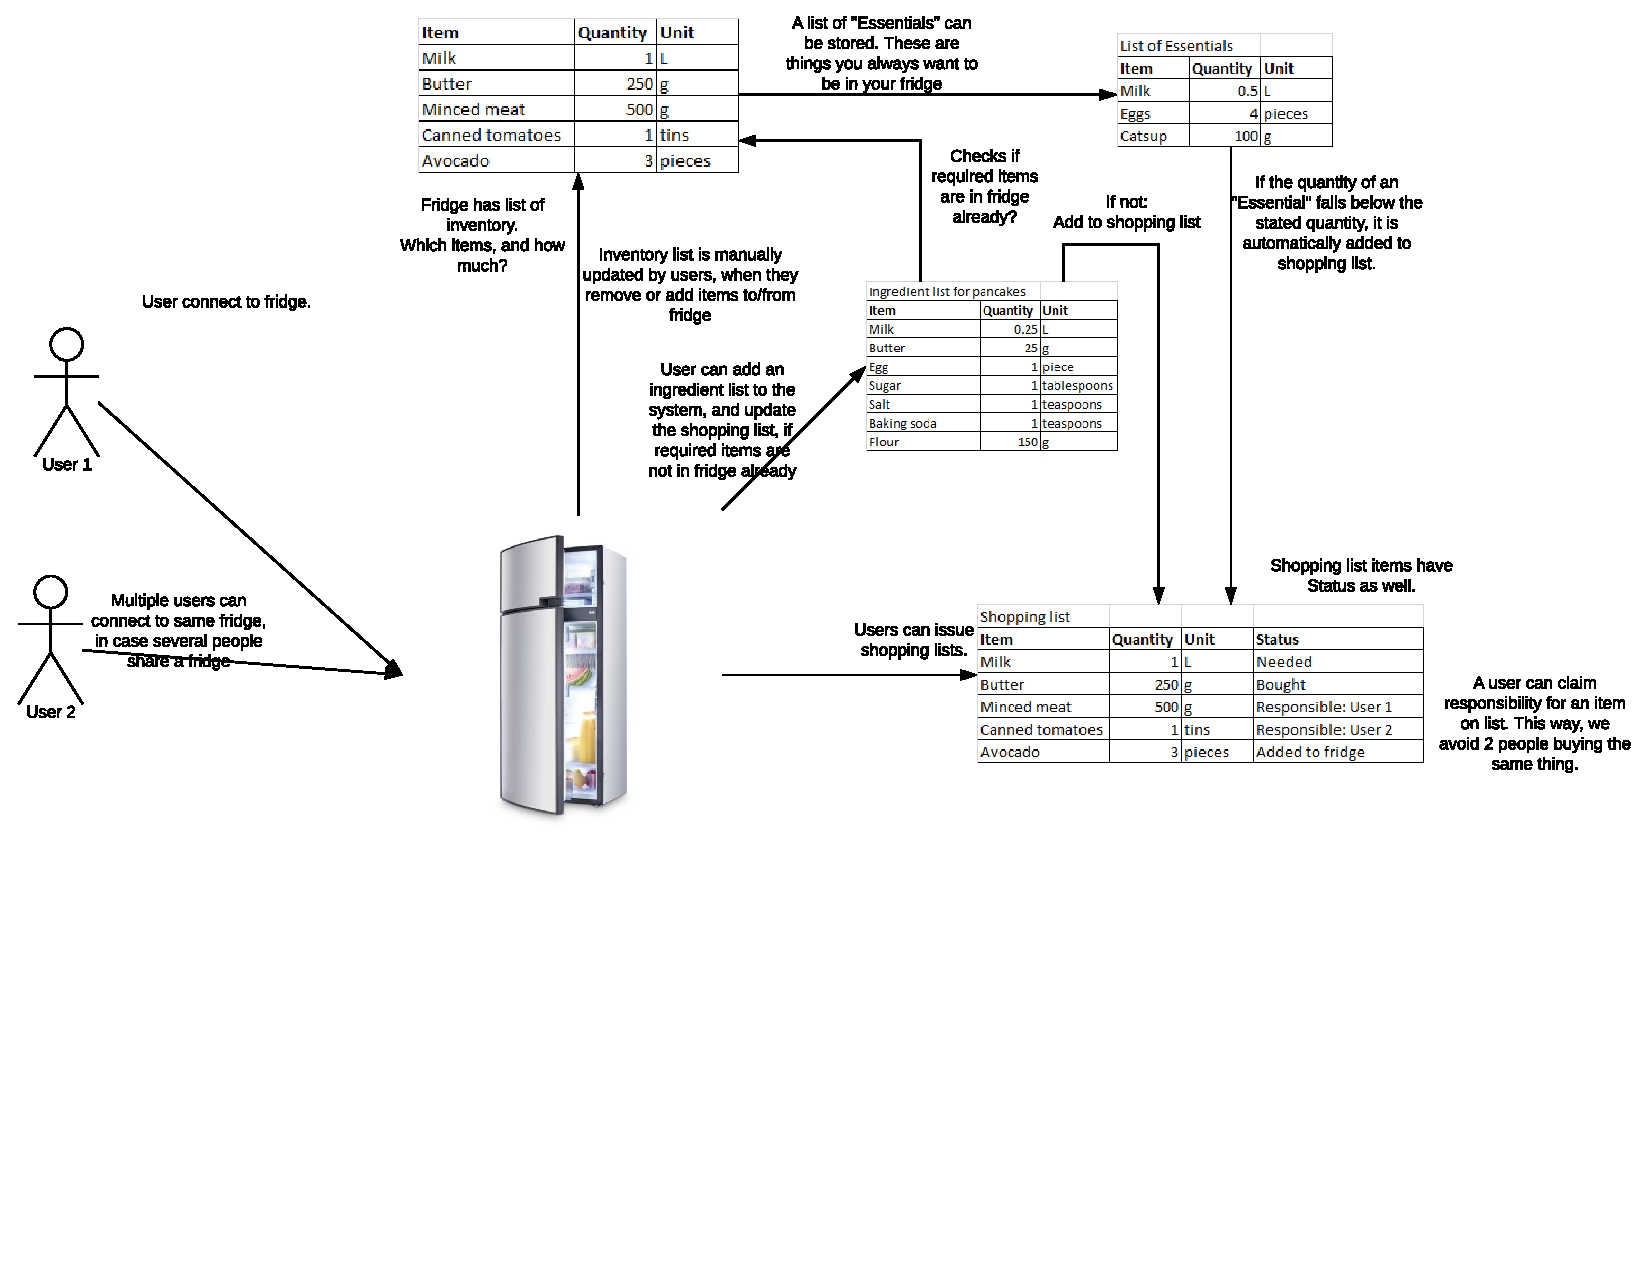
\includegraphics[width=180mm]{Img/Fridge_rich_picture.pdf}
	\caption{Rich picture of Fridge-i-nator}
	% \floatfoot{Source: (Citation command)}
	\label{fig:RichPic}
\end{figure}

\section{Early design}
Figure \ref{Design diagram} shows an early design of the system. The resulting app uses a similar structure. A notable difference however is that the service updates in real time upon changes in the database, and not periodically. This ensures that the user always has the latest data. A user profile picture was not implemented, seeing that it was not one of the first priorities. Furthermore, fridges no longer hold lists of connected users. Instead, users now have a list of fridges, that they have subscribed to. Apart from those minor changes, the overall design is the same.
\begin{figure}[H]
	\centering
	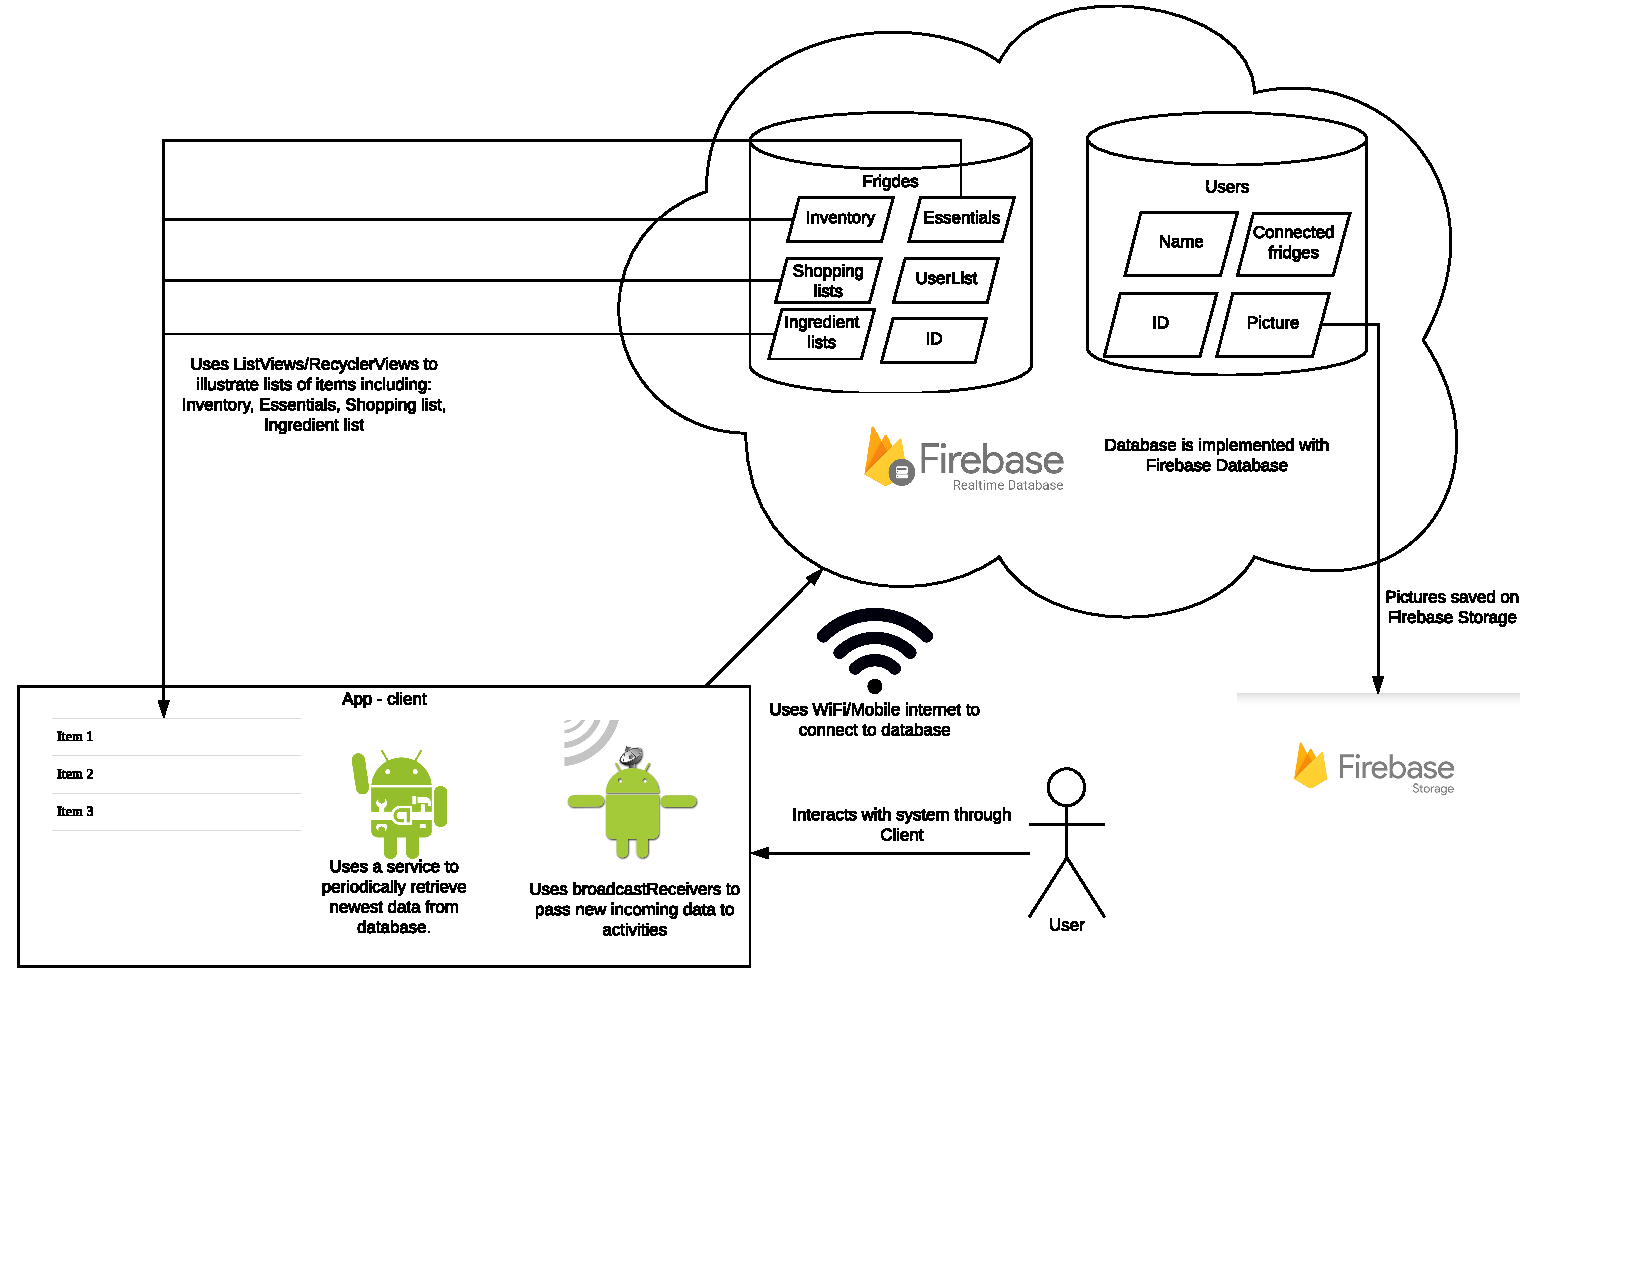
\includegraphics[width=180mm]{Img/Fridge_some_diagram.pdf}
	\caption{Early design diagram of Fridge-i-nator}
	% \floatfoot{Source: (Citation command)}
	\label{fig:Design diagram}
\end{figure}

\section{User stories}
The below user stories 

\textbf{CONNECTION}\\

As a user, I can connect to a create a new fridge, so that i can acces connect to it.

As a user, I can connect to a fridge, so that I can access information about it.

As a user, I can add other people to a fridge I am connected to, so that they can access information about it.

As a user, I can leave a fridge, so that I cannot acces information about it anymore.
\newline
\newline
\textbf{INVENTORY}

As a user, I can acces an inventory list of items which the fridges contain, so all users connected to the fridge can keep track of what is in the fridge.

As a user, I can add items to the inventory list, so that all connected users may know that the item is in the fridge.
\newline
\newline
\textbf{SHOPPING LIST}

As a user, I can acces a shopping list of items, so all users connected to the fridge can keep track of what needs to be bought for the fridge.

As a user, I can add items to the shopping list, so that all connected users may know that the item needs to be bought.
\newline
\newline
\textbf{ESSENTIALS LIST}

As a user, I can acces a list of essential items with a minimum quantity of each item, so when the quantity of at specific item comes below the minimum quantity fridge-i-nator automatically adds the item to the shopping list.

As a user, I can add items to the lsit of essential items, so that all the system automatically will add the item to the shopping list, if the quantity of the item falls below a specifiec quantity.
\newline
\newline
\textbf{INGREDIENT LIST}

As a user, I can add an ingredient list of items, so that the system will add missing items to the shopping list.
\newline
\newline
\textbf{USING THE SHOPPIN/INVENTORY LIST}

As a user, I can claim responsibility of an item on the shopping list, so that other useres will be notified about who has taken responsibility of the given item to avoid double shopping.

As a user, I can move an item from the shopping list to the inventory list, so that all users connected to the fridge will know that the item has been bought.

\subsection{Updates to the user stories}
If we look at all the user stories we made before we started the implementation of the app. These requirements are almost all met, except a couple of them. One of them was: “As a user, I can claim responsibility of an item on the shopping list, so that other useres will be notified about who has taken responsibility of the given item to avoid double shopping.” This is no longer true. Instead we decided it would be a better user experience to claim responsibility of a whole shopping list. The reason for this is that the user would waist a lot of time, claiming responsibility of each individual items he/she wants to have responsibility of buying. If the user didn’t buy all the items on the shopping list, he/she could just move the bought items to the inventory and another user could overtake the responsibility of that shopping list. 
Another feature we have implemented to improve the user experience, is if the user has bought all items in a shopping list it’s now possible to move all items to the inventory at once, instead of one at the time.  
\\
\\
Another thing we didn’t think about before we started to implement the app, was whether we wanted the app to be able to rotate. But after we had implemented the landscape mode and tried it out, it just felt like a really bad user experience. Because it gave nothing extra to the user on the contrary it just made the experience worse. It’s because our UI mainly consist of listviews and when you  turn your phone to landscape mode, its only possible to see three items in the listview at a time. Therefore the group decided to lock rotation to improve the user experience.
\\
\\
The last thing from the user stories we didn’t implement in our app was the: “As a user, I can add other people to a fridge I am connected to, so that they can access information about it.” This wasn’t implemented due to time pressure, but it would be one of the first things we would implement in future work. 


\section{Assumptions for and explanations to the chosen design}


\subsection{GUI} 
Throughout the start of the designing process of the app, there were several opinions on how the GUI could be designed, in order to achieve the best user experience. In accordance to achieving the best user experience, you would want the user to feel that the app feeling and usage is intuitive, and therefore shouldn’t raise questions about how to use it, after it being installed on the user android device. 
\\
\\
That concluded in us knowing that in order to achieve a great user experience, we needed to make the app as simple as possible in terms of a GUI.
In conclusion to the decision on focusing on a user friendly app experience, the group decided to make a GUI mockup, in order to agree on the most efficient way to build the app in order for it to make sense for the end-users. The GUI-mockup can be seen in appendix C.
\\
\\
At first time opening the app, the user will be presented with a login screen. Here the user will be asked to enter the email address. Afterwards the app will check in the Firestore database, whether the email address has been used before or this is the first time. If the email address is used for the first time, the app asks the user to select a password, which will be used in the future to log into the users account. If used before, the app simply asks for the password, unless you have setup Google Play to remember password – then it automatically log-in for you.
\\
\\
Then the user lands on the OverviewActivity, where the user will be presented a listview of fridges he/her previously has been subscribed to. Obviously that list will be empty, in case this is the first login. The user has the possibility to either create a new fridge, subscribe to an existing fridge, or to either delete or share a subscribed fridge in the listview. In addition, the user can choose to press a fridge on the listview to go to the fragmentview, DetailsActivity, to see details for the choosen fridge.
\\
\\
The fragment view concludes 4 different tabs, where each of the holds separate information presented in a listview. There is an inventory list, which concludes the things that the user currently has on shelves/in fridge. The essentials-list, where the user can define which items they never want to go below a given threshold. If that threshold is reached, it will automatically be added to the shoppinglist. The user can access each different shoppinglist and see what items and quantity they hold. Ingredientlists is the last tab, and it holds a list of known recipes, which the user can press and see what is needed to make the specific recipe. The possibility to add further items to the recipe and add the total list of items needed for the recipe to the shoppinglist.
As stated, the above, has been the outline of the GUI designed and thereafter been carried out within the development-process of the app.
\\
\\
\subsection{Fragments}
Due to the group wanting a great user experience troughout the app, there was a need for us to display the relevant data to the user, in the best possible way.
We concluded that one of the best solutions would be in a fragmented view, which listed 4 tabs: Inventory, Essentials, Shoppinglists and IngredientsList.
Thereby the user can quickly access the data and switch beetween the list, depending on what the user intend to do, whether he/she wants to go to shoppinglists to add all items to inventory, or seemleesly check an ingredientslist.
\\
\\
The fragmented views normally comes as one single class. Since the group felt there was an slight chance there could become to much chaos in the loop of creating and switching from tab to tab inside one single class (DetailsActivity), we therefor decided to split up each tab into their own single class.
\\
\\
Then we implemented the functionality in the detailsActivity so they would display the correct tabs and refer to the tabs individual class.
In each class it extends Fragment and a onCreateView class, which inflates the correct tab .xml file, in order to show the correct UI information to the user.
\\
\\
The outline and outcome of this decision have maked the development of the fragtment activities easier than normal, without compromising the users user interface experience.

\subsection{Data Access Layer}
As database for this project, we are using firestore by firebase. This was chosen because it offers an easy-to-use database solution which is highly integrable with Android. It provides the capability to add “EventListeners” to documents and collections in the database, which will trigger events in the code. This provides us with a sort of observer pattern, where the individual devices subscribed to the database can receive new data, when it is changed in the database.
\\
\\
The Data Access Layer is split into 2 parts:\\ \textbf{fireStoreCommunicator}: handles the lowest level of communication with the database. This includes adding new lists, adding items to list, adding users to database, subscribing to fridges, receiving data, making lists from this data, etc…
\\
\\
\textbf{ServiceUpdater}: this serves as the Programming Interface throughout the app. The service also holds a local copy of all fridges the user has subscribed to. All actions done in the activities/fragments goes through the service. For instance, when adding an item to a list in an activity, the service checks if an item with matching name is already on the list. If so, it increments the quantity of that item in the database, instead of adding a duplicate item.
From the service, we send out a broadcast whenever the service has retrieved new data from the database. This way, the activities/fragments can retrieve the newest data from the service, and thus stay in sync with the database.
The reason for choosing the approach where the service holds a local list of the data in the database is because we had experience with this approach from the Assignment 2.

One could argue that it is bad programming practice to have such a huge amount of logic in these 2 classes, and that we instead should have divided the functionality into several lesser classes. Had we had more time, a rework of the architecture would be a topic of high priority.

\subsubsection{Data flow}
Figure \ref{fig:dataflow_diagram} shows a conceptual diagram of the data flow. It should be noted that when a user for instance adds an item to a list, the change does not take effect locally, before it has been added to the database. This ensures that the database and the app stays in sync. The drawback of this is that items cannot be added if the database cannot be accessed at the time of use.
\begin{figure}[H]
	\centering
	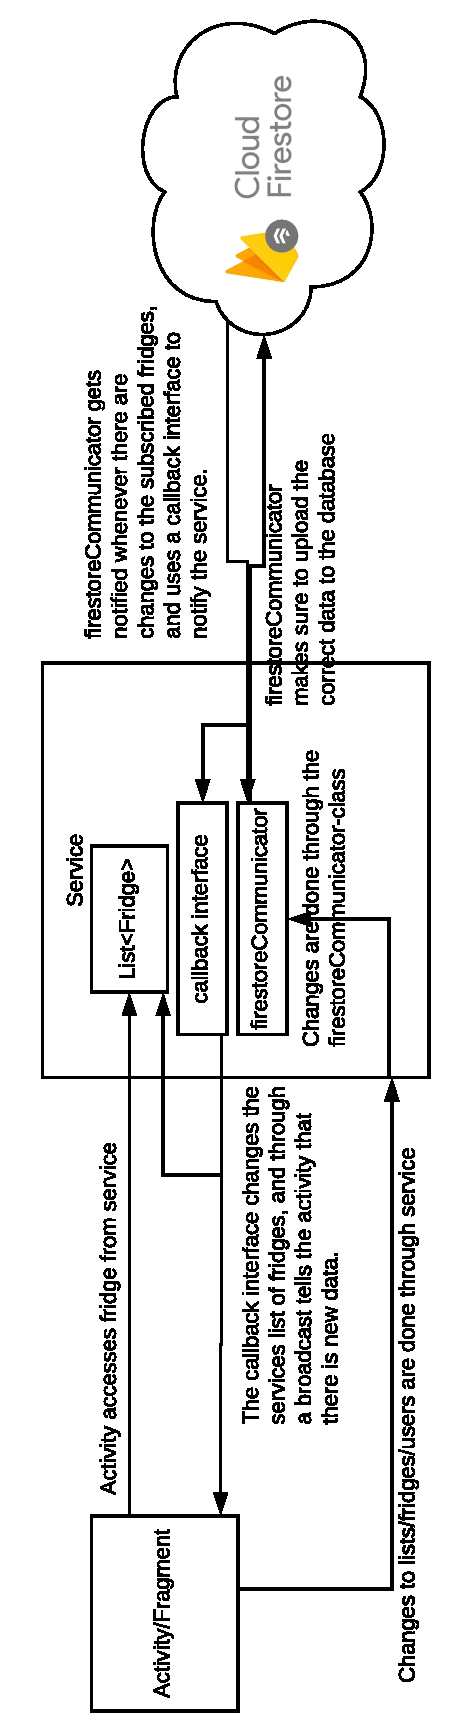
\includegraphics[width=180mm]{Img/SMAP_DAL}
	\caption{Conceptual diagram of data flow of Fridge-i-nator}
	% \floatfoot{Source: (Citation command)}
	\label{fig:dataflow_diagram}
\end{figure}

\textbf{Sequence Diagrams}
Appendices A and B show 2 sequence diagrams. One shows the process of adding an item to a list through the service, and in turn the firestoreCommunicator.
The other diagram shows the process of updating the UI, when data on one of the subscribed lists are updated.
As example, we are showing the inventory list, but managing the other lists are basically the same.\\


\textbf{Authentication}
\\
For user authentication we used firebaseUI, which provides an easy to use solution for authentification with a variety of different social media integration as well. We chose to keep it simple and use authentification via email and password.
\\
\\
\textbf{Authorization}
\\
As of now, proper user authorization has not been implemented yet. This means that the database is open for reading and writing for anyone. This is of course not optimal, but given the scope of the assignment, this was not prioritized.

\subsection{Adaptors}
The UI manly consist of listviews and all these listviews use separate listview adaptors. We found inspiration from lection 4 to make these adaptors. The reason why we use separate listview adaptors for every fragment and activity, is to make it easy to customize the listviews, and that way improve the user experience. Eg. the shoppinglist shows the name of the shopping list and who's responsible, and the inventory list shows the name, quantity and unit of the items. This works well with the on click options the user has eg. click on an item to adjust the quantity of that item, or to make a long click on an item to get the option to delete an item.

\section{Future work}
Had the group had more time the following would be points of improvement and further work.
\begin{itemize}
	\item \textbf{Authorization} - As of now, the database is open for everyone. This is of course sub-optimal. Only users connected to the fridge should be able to read and write data.
	\item \textbf{Notifications} - A useful feature would be that users responsible for a given shopping list would receive notification, if there were changes to the shopping list.
	\item \textbf{Stability} - As of now, sometimes the app will not update the UI immediately upon changes in the database. This would of course be a major focus, as it is a core part of the user experience and general fluency of the app.
	\item \textbf{Share fridge ID} - As of now, when the use wants to share the fridge, the ID is just displayed as a message. It would be nice to be able to send it via messenger or copy it to clipboard instead.
\end{itemize}

\section{Conclusion}
In conclusion of all the thoughts that went into the design and architecture of the code, has resulted in a app that generally fulfils the idea of what the app was meant to be. We have created a app that enables the family-members, roomies and others, to have an easier life in terms of going grocery-shopping. In light of bugs and other know problems, there is still space for improvement in the app – even though the main ability and purpose of the app is working as intended – which indeed is to make grocery-shopping an easier part of the users day. The group has several points of view in terms of functionality which could be implemented in future work, which in the end would make the app and its functionality even more desirable to the user, and thereby creating a better user experience. The group members have indeed as well fulfilled several of our own personal Android Development goal and personal visions, which also has been a fulfilling result of this app project. Therefore we conclude this project as a successful implementation with a few beauty-faults and room future work in terms of functionality and user experience improvements.

\section{Bugs and known problems}

\begin{easylist}
	& If quantity of an item is given a very(very) large value, it changes value to "infinity". If you change quantity for the same item again, you can input a number + the word "infinity", which crashes the app.
	\\
	\\	
	& General stability problems.
	\\
	\\
	& Layout not matching all screen sizes.
	\\
	\\
	& When creating a new fridge name is displayed as null. It is however displayed correctly when the app is restarted.
\end{easylist}

\pagebreak
\section{Appendix}
PLEASE NOTE: All images in Appendix can be found along with the report as well.
\subsection{Appendix A: Sequence diagram - Add item}
\begin{figure}[H]
	\centering
	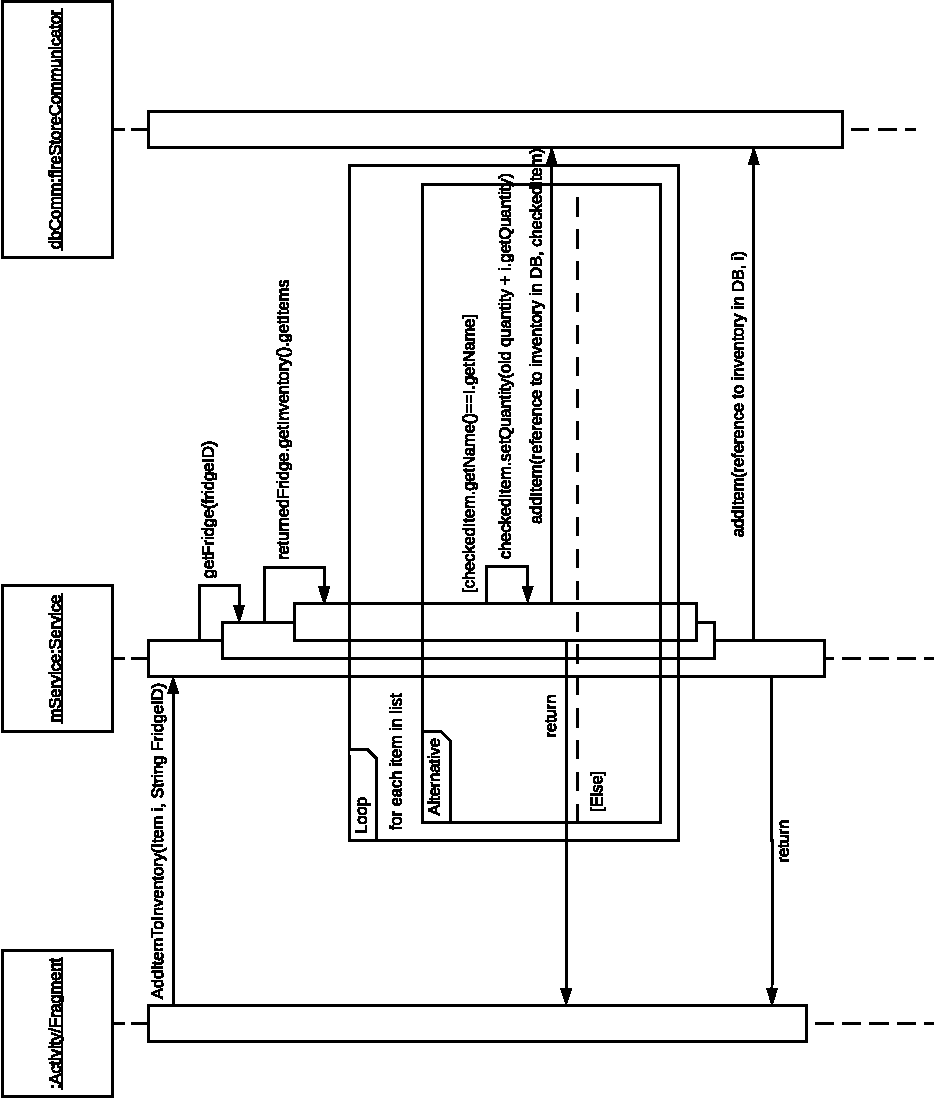
\includegraphics[width=180mm]{Img/APPENDIX A - SD-ADD-ITEM.pdf}
	\caption{Sequence diagram of adding a new item to inventory - PLEASE NOTE: All images in Appendix can be found along with the report as well.}
	% \floatfoot{Source: (Citation command)}
	\label{fig:SD_addItem}
\end{figure}

\subsection{Appendix B: Sequence diagram - Update UI on new data for subscribed list}
\begin{figure}[H]
	\centering
	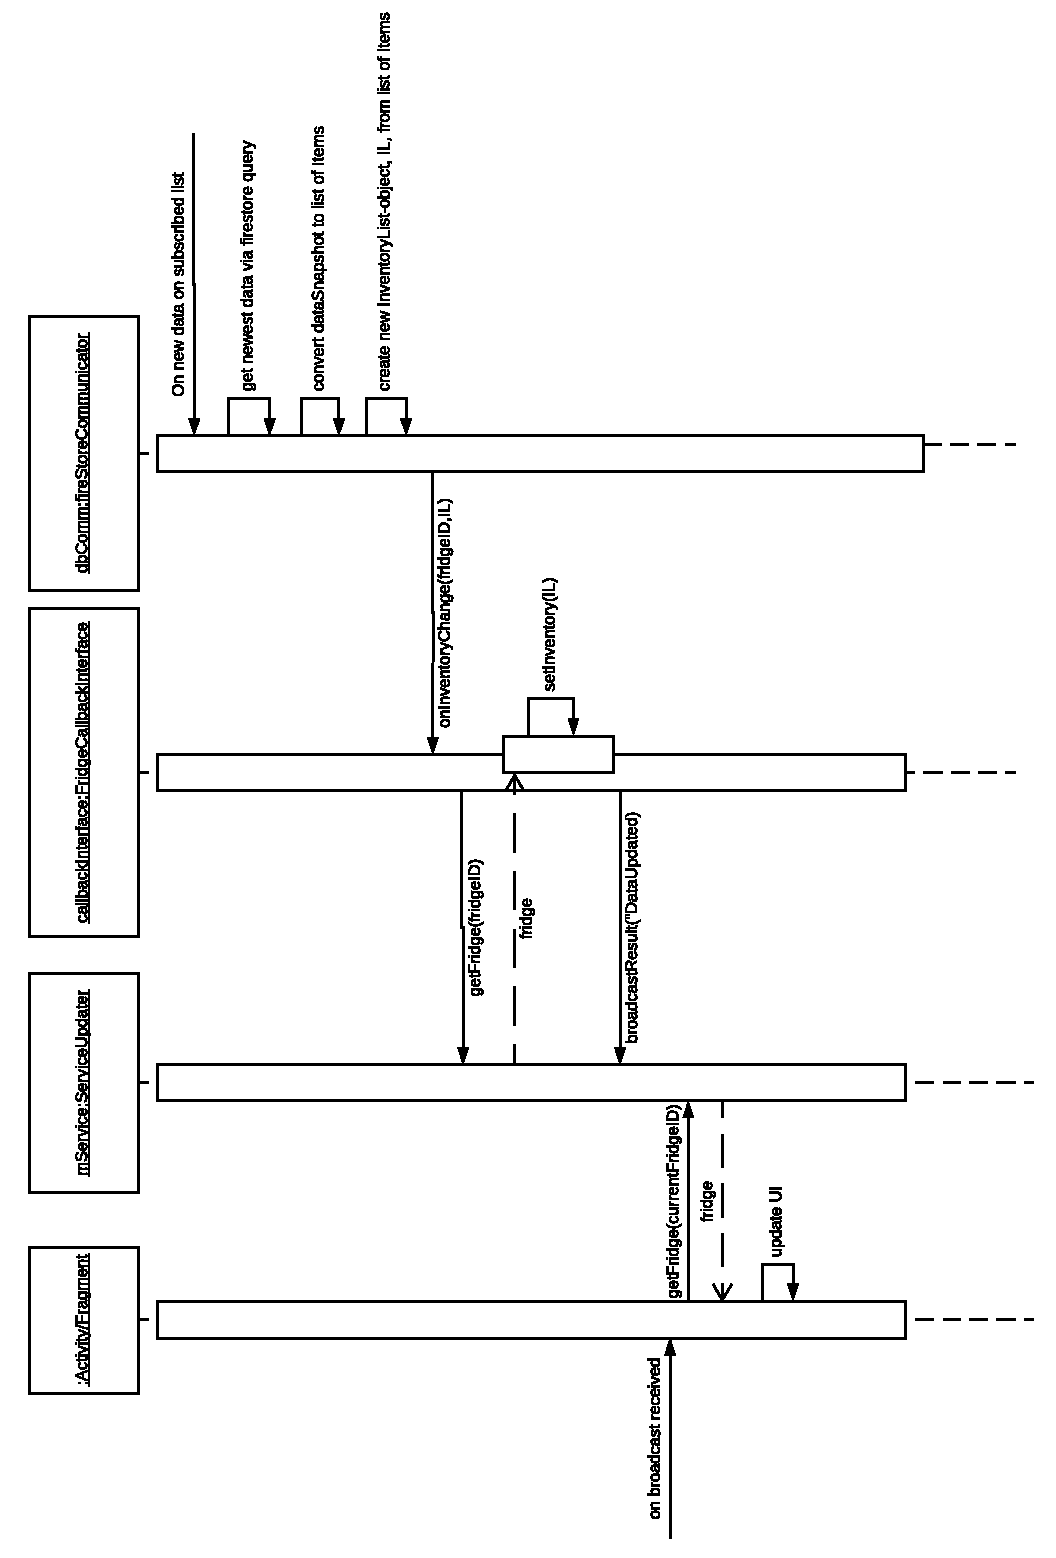
\includegraphics[width=120mm]{Img/APPENDIX B - SD-onNewData.pdf}
	\caption{Sequence diagram of updating UI upon receiving new data in the database. - PLEASE NOTE: All images in Appendix can be found along with the report as well.}
	% \floatfoot{Source: (Citation command)}
	\label{fig:SD_onNewData}
\end{figure}

\subsection{Appendix C: GUI mockup}
\begin{figure}[H]
	\centering
	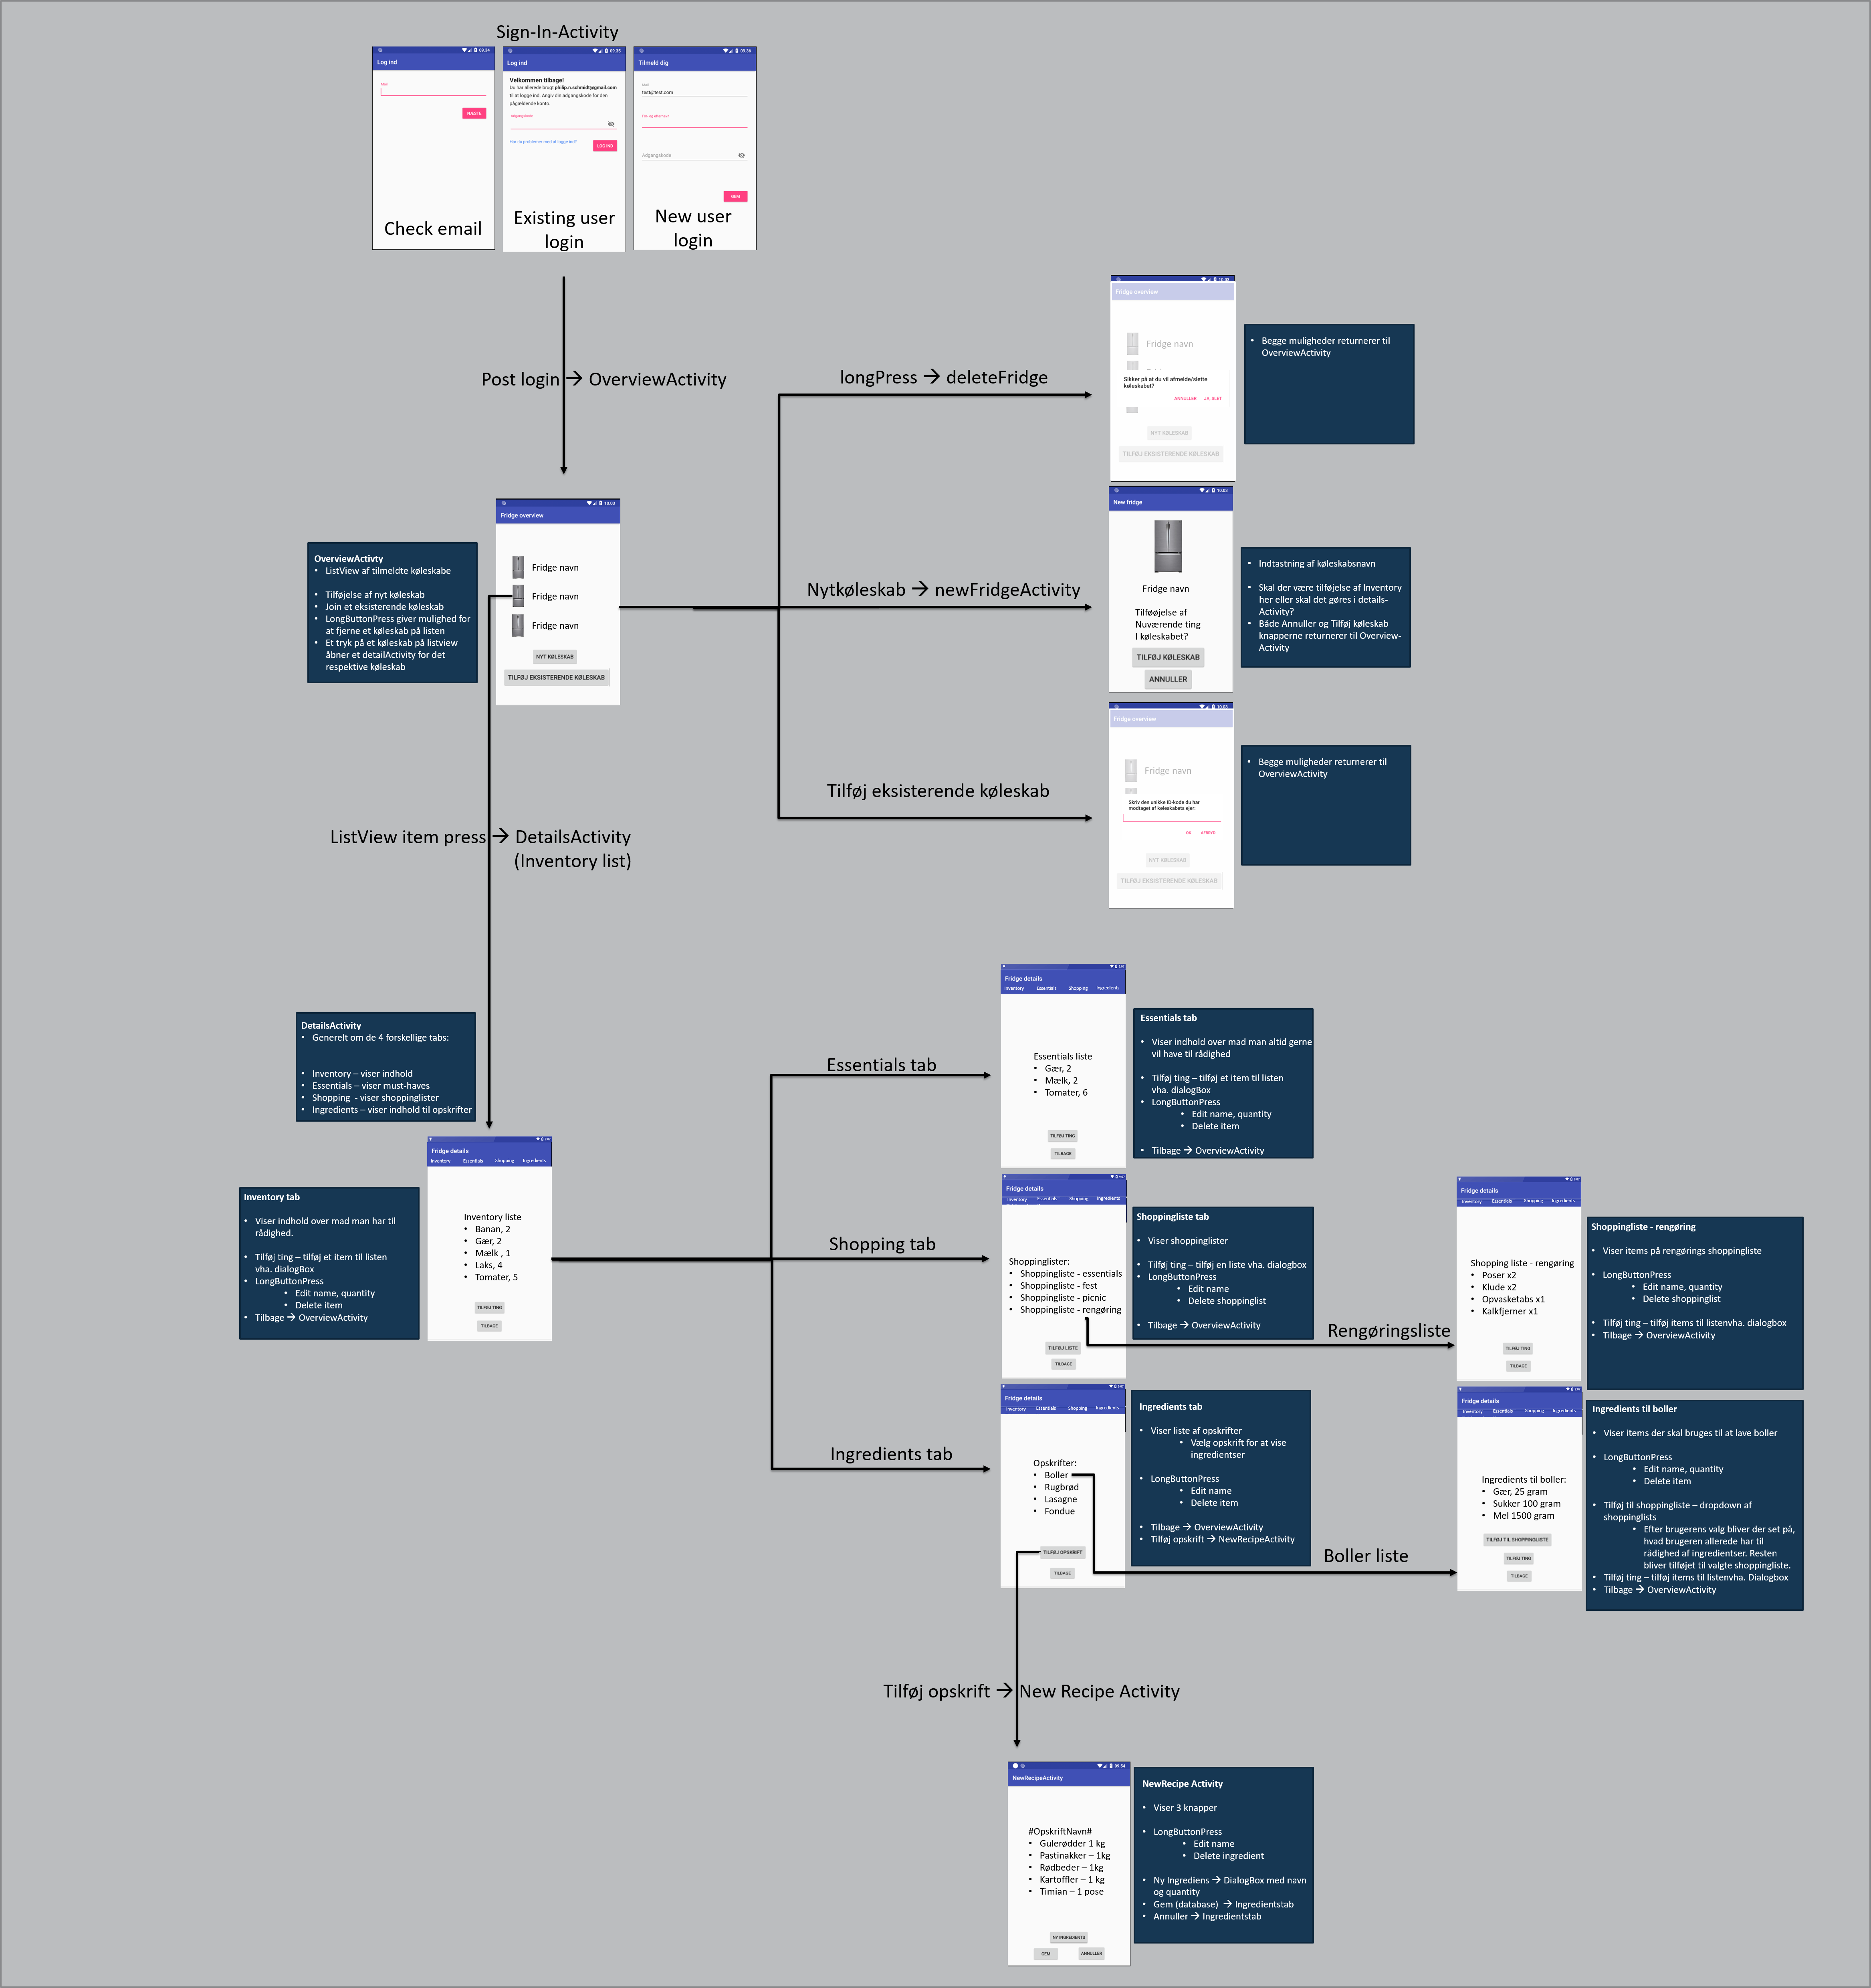
\includegraphics[width=180mm]{Img/APPENDIX C - GUI-mockup.png}
	\caption{Early draft of the UI - PLEASE NOTE: All images in Appendix can be found along with the report as well.}
	% \floatfoot{Source: (Citation command)}
	\label{fig:GUI_mockup}
\end{figure}

\end{document}

